% Claudia Porto, COMPLETE

Graph theory is fundamental in understanding the various graph structures that arise in problems like maximum matching. The structure of the graph significantly influences both the choice of algorithm and its efficiency. By providing essential principles and techniques, graph theory equips us to navigate different graph types and select the most appropriate algorithms for solving matching problems. This understanding is crucial for addressing the challenges posed by diverse graph scenarios and developing efficient, specialized algorithms for maximum matching in various settings.

\subsection{Graphs}
A \textbf{graph} \( G \) is defined as an ordered pair \( G = (V, E) \), where:
\begin{itemize}
    \item \( V \) is an finite set of \textbf{vertices}.
    \item \( E \) is a set of \textbf{edges}, where each edge is an unordered pair of distinct vertices \( u, v \in V \), where \( E \subseteq [V^2]\).
    \begin{itemize}
        \item \([V^2] = V \times V\)
        \item \(V^d = V_1 \times V_2 \times ... \times V_d\)
    \end{itemize}
\end{itemize}
Depending on the context, sometimes graphs are called \textbf{networks}, vertices are called \textbf{nodes}, and edges are called \textbf{arcs}. In a graph, no two edges are identical, between any pair of vertices, there is at most one edge, and there can be \textbf{self loops}, edges of the form \( \{v, v\} \) where a vertex is connected to itself.

For example, consider the graph \( G = (V, E) \) in Figure~\ref{fig:general_graph}:
\[
V = \{1, 2, 3\}, \quad E = \{\{1, 2\}, \{2, 3\}\}
\]

\begin{figure}[h]
\begin{center}
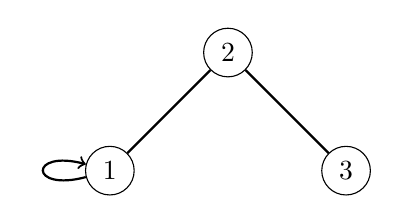
\begin{tikzpicture}[scale=1.5]
    % Draw nodes
    \node[circle, draw] (1) at (0, 0) {1};
    \node[circle, draw] (2) at (1, 1) {2};
    \node[circle, draw] (3) at (2, 0) {3};

    % Draw edges
    \draw[thick] (1) -- (2);
    \draw[thick] (2) -- (3);
    \draw[thick, ->] (1) to[loop left] (1);
\end{tikzpicture}
\caption{A graph with three vertices, two edges, and a self-loop at vertex 1.}
\label{fig:general_graph}
\end{center}
\end{figure}

This represents a graph with three vertices $V = 1, 2, 3$, and two edges connecting vertices 1 and 2, and vertices 2 and 3 with a self loop on vertex 1.\cite{yadav2023advanced, cormen2009introduction}

Graphs can be categorized as either \textbf{undirected} or \textbf{directed}, depending on whether their edges are bidirectional or have a specific direction. 

In an \textbf{undirected graph}, an edge between vertices \( u \) and \( v \) is represented as \( \{u, v\} \), indicating that the edge can be traversed in either direction. An undirected graph is defined as:
\[
G = (V, E) \quad \text{where} \quad E \subseteq \{\{u, v\} \mid u, v \in V, u \neq v \}
\]

In Figure~\ref{fig:undirected_graph}, all edges are bidirectional and can be written as \{\{1,2\}, \{2,3\}, \{1,3\}\} or \{\{2,1\}, \{3,2\}, \{3,1\}\}, among other permutations. All of these are equivalent representations because the order of vertices in an edge does not matter in an undirected graph.

\begin{figure}[h]
\begin{center}
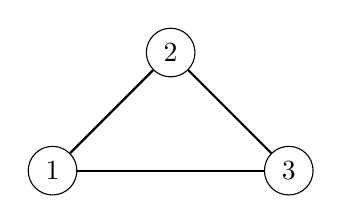
\begin{tikzpicture}[scale=1.5]
    % Draw nodes
    \node[circle, draw] (1) at (0, 0) {1};
    \node[circle, draw] (2) at (1, 1) {2};
    \node[circle, draw] (3) at (2, 0) {3};

    % Draw edges (undirected)
    \draw[thick] (1) -- (2); % Edge between 1 and 2
    \draw[thick] (2) -- (3); % Edge between 2 and 3
    \draw[thick] (1) -- (3); % Edge between 1 and 3
\end{tikzpicture}
\caption{An undirected graph with bidirectional edges connecting vertices 1, 2, and 3.}
\label{fig:undirected_graph}
\end{center}
\end{figure}

In a \textbf{directed graph}, each edge has a specific direction. An edge from vertex \( u \) to vertex \( v \) is denoted by \( (u, v) \), and the edge can only be traversed from \( u \) to \( v \). A directed graph is defined as:
\[
G = (V, E) \quad \text{where} \quad E \subseteq \{(u, v) \mid u, v \in V, u \neq v \}
\]

In this case, \( (u, v) \) is an ordered pair, and the directionality of the edge imposes a one-way relationship from \( u \) to \( v \). For example, consider a directed graph \( G = (V, E) \) in Figure~\ref{fig:directed_graph} where:
\[
V = \{1, 2, 3\}, \quad E = \{(1, 2), (2, 3)\}
\]

\begin{figure}[h]
\begin{center}
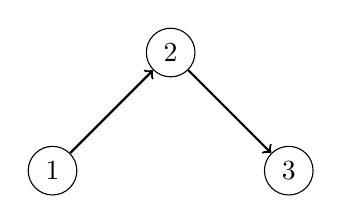
\begin{tikzpicture}[scale=1.5]
    % Draw nodes
    \node[circle, draw] (1) at (0, 0) {1};
    \node[circle, draw] (2) at (1, 1) {2};
    \node[circle, draw] (3) at (2, 0) {3};

    % Draw directed edges
    \draw[thick,->] (1) -- (2); % Directed edge from 1 to 2
    \draw[thick,->] (2) -- (3); % Directed edge from 2 to 3
\end{tikzpicture}
\caption{A directed graph with edges from vertex 1 to 2 and vertex 2 to 3}
\label{fig:directed_graph}
\end{center}
\end{figure}

In this graph, there is a directed edge from vertex 1 to vertex 2, and another directed edge from vertex 2 to vertex 3. \cite{yadav2023advanced, cormen2009introduction}

\subsection{Weighted Graphs}

A \textbf{weighted graph} is a graph in which each edge is assigned an integer, known as the \textbf{weight} of the edge. The weight typically represents a cost, distance, or any measurable attribute of the connection between two vertices.\cite{mathew2017weighted}

Each edge in a weighted graph can be represented by a tuple \((u, v, w)\), where:
\begin{itemize}
    \item \( u \) and \( v \) are vertices connected by the edge.
    \item \( w \) is the weight of the edge between \( u \) and \( v \).
\end{itemize}
Since the graph in this example is undirected, the order of $u$ and $v$ does not matter; the edge \((u,v,w)\) is equivalent to \((v,u,w)\). However, the weight $w$ is always the last part of the tuple and uniquely identifies the value associated with the connection.

For example, consider the weighted graph in Figure~\ref{fig:weighted_graph} where:
\[
V = \{1, 2, 3, 4\}, \quad E = \{(1, 2, 3), (1, 3, 2), (2, 3, 4), (3, 4, 5), (1, 4, 1)\}
\]

\begin{itemize}
    \item The vertices \( V \) represent nodes labeled \( 1 \) through \( 4 \).
    \item The edges \( E \) are tuples that specify the connection between two vertices and their associated weights. For instance, the edge \( (1, 2, 3) \) indicates a connection between vertices \( 1 \) and \( 2 \) with a weight of \( 3 \).
\end{itemize}

Figure~\ref{fig:weighted_graph} visually represents the graph. Each node corresponds to a vertex, and each line connecting two nodes represents an edge labeled with its respective weight. For example:
\begin{itemize}
    \item The edge between vertex \( 1 \) and vertex \( 4 \) has a weight of \( 1 \).
    \item The edge between vertex \( 3 \) and vertex \( 4 \) has a weight of \( 5 \).
\end{itemize} 

\begin{figure}[h]
\begin{center}
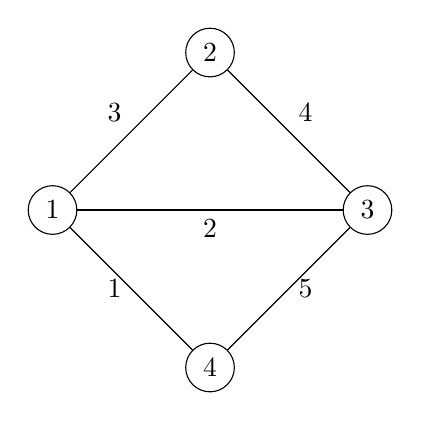
\begin{tikzpicture}
    % Nodes
    \node[draw, circle] (v1) at (0, 0) {1};
    \node[draw, circle] (v2) at (2, 2) {2};
    \node[draw, circle] (v3) at (4, 0) {3};
    \node[draw, circle] (v4) at (2, -2) {4};
  
    % Edges with weights
    \draw[-] (v1) -- node[above left] {3} (v2);
    \draw[-] (v1) -- node[below] {2} (v3);
    \draw[-] (v2) -- node[above right] {4} (v3);
    \draw[-] (v3) -- node[right] {5} (v4);
    \draw[-] (v1) -- node[left] {1} (v4);
\end{tikzpicture}
\caption{A weighted graph with vertices V = 1, 2, 3, 4 and their corresponding weighted edges}
\label{fig:weighted_graph}
\end{center}
\end{figure}

\subsection{Adjacent Vertices and Incident Edges}

Two vertices \( u \) and \( v \) in a graph \( G \) are called \textbf{adjacent} if they are joined by an edge. In an undirected graph, this means \( \{u, v\} \in E(G) \), while in a directed graph, \( u \) is adjacent to \( v \) if \( (u, v) \in E(G) \).

For example, in the undirected graph \( G = (V, E) \) in Figure~\ref{fig:adj_vertices}, where \( V = \{1, 2, 3\} \) and \( E = \{\{1, 2\}, \{2, 3\}\} \), vertices 1 and 2 are adjacent (in red), and vertices 2 and 3 are adjacent (in blue).

\begin{figure}[h]
\begin{center}
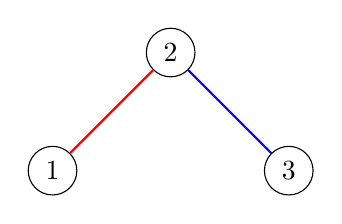
\begin{tikzpicture}[scale=1.5]
    % Draw nodes
    \node[circle, draw] (1) at (0, 0) {1};
    \node[circle, draw] (2) at (1, 1) {2};
    \node[circle, draw] (3) at (2, 0) {3};

    % Draw edges with different colors
    \draw[thick, red] (1) -- (2); % Edge from node 1 to node 2 in red
    \draw[thick, blue] (2) -- (3); % Edge from node 2 to node 3 in blue
\end{tikzpicture}
\caption{An undirected graph showing adjacency between vertices, with edges colored to indicate adjacency relations.}
\label{fig:adj_vertices}
\end{center}
\end{figure}

An edge \( e \) is said to be \textbf{incident} to the vertices it joins. In an undirected graph, if \( e = \{u, v\} \), then \( e \) is incident to both \( u \) and \( v \). In a directed graph, if \( e = (u, v) \), then the edge is incident to \( u \) as an outgoing edge and to \( v \) as an incoming edge.  \cite{yadav2023advanced, cormen2009introduction}

\subsection{Degree of a Vertex}
\vspace{0.05cm}
In an undirected graph, the \textbf{degree} of a vertex \( v \) is the number of edges incident to \( v \), denoted by \( \deg(v) \). \cite{yadav2023advanced, cormen2009introduction} On the other hand, in a directed graph, the degree is split into two parts:
\begin{itemize}
    \item \textbf{In-degree}: The number of edges directed into the vertex \( v \), denoted by \( \deg^-(v) \).
    \item \textbf{Out-degree}: The number of edges directed out of the vertex \( v \), denoted by \( \deg^+(v) \).
\end{itemize}

For example, in the graph \( G = (V, E) \) in Figure~\ref{fig:degree} with \( V = \{1, 2, 3\} \) and \( E = \{\{1, 2\}, \{2, 3\}\} \), the degree of vertex 2 is 2, since it is connected to both vertices 1 and 3.

\begin{figure}[h]
\begin{center}
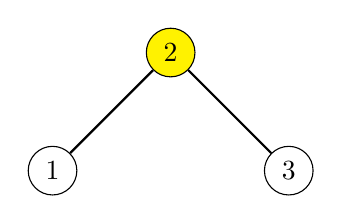
\begin{tikzpicture}[scale=1.5]
    % Draw nodes
    \node[circle, draw] (1) at (0, 0) {1};
    \node[circle, draw, fill=yellow] (2) at (1, 1) {2}; % Highlighted vertex 2 with a fill color
    \node[circle, draw] (3) at (2, 0) {3};

    % Draw edges
    \draw[thick] (1) -- (2);
    \draw[thick] (2) -- (3);
\end{tikzpicture}
\caption{An undirected graph illustrating the degree of vertex 2, highlighted in yellow.}
\label{fig:degree}
\end{center}
\end{figure}

In a directed graph \( G = (V, E) \) in Figure~\ref{fig:directed_degree} with \( V = \{1, 2, 3\} \) and \( E = \{(1, 2), (2, 3)\} \), the in-degree and out-degree of vertex 2 are as follows:
\begin{itemize}
    \item \(\deg^-(2) = 1\) (one edge points into vertex 2)
    \item \(\deg^+(2) = 1\) (one edge points out to vertex 3)
    \item \(\deg^-(1) = 0\)
\end{itemize}

\begin{figure}[h]
\begin{center}
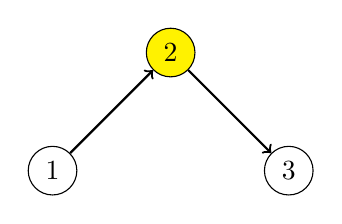
\begin{tikzpicture}[scale=1.5]
    % Draw nodes
    \node[circle, draw] (1) at (0, 0) {1};
    \node[circle, draw, fill=yellow] (2) at (1, 1) {2}; % Highlighted vertex 2 with a fill color
    \node[circle, draw] (3) at (2, 0) {3};

    % Draw directed edges
    \draw[thick,->] (1) -- (2); % Directed edge from 1 to 2
    \draw[thick,->] (2) -- (3); % Directed edge from 2 to 3
\end{tikzpicture}
\caption{A directed graph showing the in-degree and out-degree of vertex 2, highlighted in yellow.}
\label{fig:directed_degree}
\end{center}
\end{figure}

\subsection{Bipartite Graphs}
Let \( V \) be a set of vertices, \( d = 2 \) be an integer, and \( G = (V, E) \) be a bipartite graph. A \textbf{bipartite graph} is a graph where the vertex set \( V \) can be partitioned into two disjoint sets \( V_1 \) and \( V_2 \) such that every edge in \( E \) connects a vertex in \( V_1 \) to a vertex in \( V_2 \). In other words, no two vertices within the same set are adjacent.  \cite{yadav2023advanced}

Formally, \( V = V_1 \cup V_2 \) and \( V_1 \cap V_2 = \emptyset \), with every edge \( e \in E \) satisfying \(e \subseteq V_1 \times V_2\). This means that each edge is a pair \(v_1, v_2\), where \( v_1 \in V_1 \) and \( v_2 \in V_2 \). For example, the following graph in Figure~\ref{fig:bipartite} is bipartite:
\[
V = \{1, 2, 3, 4\}, \quad E = \{\{1, 3\}, \{2,3\}, \{2, 4\}\}
\]

\begin{figure}[h]
\begin{center}
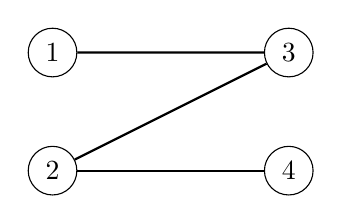
\begin{tikzpicture}[scale=1.5]
    % Draw nodes
    \node[circle, draw] (1) at (0, 1) {1};
    \node[circle, draw] (2) at (0, 0) {2};
    \node[circle, draw] (3) at (2, 1) {3};
    \node[circle, draw] (4) at (2, 0) {4};

    % Draw edges
    \draw[thick] (1) -- (3);
    \draw[thick] (2) -- (3);
    \draw[thick] (2) -- (4);
\end{tikzpicture}
\caption{An example of a bipartite graph}
\label{fig:bipartite}
\end{center}
\end{figure}

In Figure~\ref{fig:bipartite}, \( G = (V, E) \), where \( V = \{1, 2, 3, 4\} \), and the edge set is \( E = \{\{1, 3\}, \{2, 3\}, \{2, 4\}\} \). This graph satisfies the condition that every edge connects a vertex from \( V_1 \) to a vertex from \( V_2 \), and no edge connects two vertices within the same set.

\subsection{Hypergraphs}
A \textbf{hypergraph} \( H = (V, E) \) is a generalization of a graph, where \( V \) is the set of vertices and \( E \) is the set of \textbf{hyperedges}. Unlike in traditional graphs, where each edge connects exactly two vertices, a hyperedge in a hypergraph can connect any number of vertices. More formally, each hyperedge is a subset of \( V \), which may contain more than two elements \cite{cormen2009introduction}.

For example, consider a hypergraph \( H = (V, E) \) in Figure~\ref{fig:hypergraph} where:
\[
V = \{1, 2, 3, 4\}, \quad E = \{\{1, 2\}, \{2, 3, 4\}\}
\]
Here, the hyperedge \( \{1, 2\} \) connects vertices 1 and 2, and the hyperedge \( \{2, 3, 4\} \) connects vertices 2, 3, and 4. The key distinction from traditional graphs is that a hyperedge can contain more than two vertices, as seen with \( \{2, 3, 4\} \), which connects three vertices simultaneously. This capability enables hypergraphs to model more intricate relationships, such as multi-way interactions, which cannot be easily captured by standard graphs.

\begin{figure}[h]
\begin{center}
\begin{tikzpicture}
    % Draw nodes
    \node (v1) at (0,0) [draw, circle, inner sep=2pt] {$1$};
    \node (v2) at (1.5,2) [draw, circle, inner sep=2pt] {$2$};
    \node (v3) at (3,0) [draw, circle, inner sep=2pt] {$3$};
    \node (v4) at (3,2) [draw, circle, inner sep=2pt] {$4$};

    % Hyperedges
    \begin{scope}[fill opacity=0.5]
    % Hyperedge connecting 2, 3, and 4
    \filldraw[fill=yellow!70] 
        ($(v2)+(-0.5,0)$) 
        to[out=90,in=180] ($(v4) + (1,0.5)$) 
        to[out=0,in=90] ($(v3) + (0,-1)$)
        to[out=270,in=0] ($(v4) + (0,-3)$)
        to[out=180,in=270] ($(v2)+(-0.5,0)$);
    
    % Hyperedge connecting 1 and 2
    \filldraw[fill=blue!70] 
        ($(v1)+(-0.5,-0.2)$) 
        to[out=90,in=180] ($(v2) + (0.5,0.5)$) 
        to[out=0,in=90] ($(v1)+(0.4,-0.2)$)
        to[out=270,in=0] ($(v1)+(-0.5,-0.2)$);
    \end{scope}

    % Labels for hyperedges
    \node at (2, 3) {$e_2 = \{2, 3, 4\}$};
    \node at (0, -1) {$e_1 = \{1, 2\}$};
\end{tikzpicture}
\caption{An example of a hypergraph}
\label{fig:hypergraph}
\end{center}
\end{figure}

Hypergraphs are particularly useful in problems that involve complex sets and relationships, such as:
\begin{itemize}
    \item \textbf{3D Matching}: In this problem, the goal is to find a matching between sets of vertices, where each matching involves three vertices rather than two, naturally fitting the framework of hypergraphs.
    \item \textbf{Set Cover}: Hypergraphs can be used to represent set cover problems, where each hyperedge corresponds to a set, and the goal is to cover the entire vertex set using the fewest number of hyperedges.
\end{itemize}

In contrast to traditional graphs, where edges simply represent pairwise connections, hypergraphs can represent more general relationships between sets of vertices, making them a powerful tool in the study of combinatorial structures and optimization problems.

\subsection{D-Partite Graphs} 
Let \( V \) be a set, \( d \geq 2 \) be an integer, and \( G = (V, E) \) be a d-partite graph, where \(V = V_1 \cup V_2 ... \cup V_d\) and \(E \subseteq V_1 \times V_2 \times ... \times V_d\). A \textbf{d-partite graph} \( G = (V, E) \) is a type of hypergraph where the vertex set \( V \) can be partitioned into \( d \) disjoint sets \( V_1, V_2, \dots, V_d \) such that no two vertices within the same set are adjacent. Edges have exactly one vertex from each set. For example, consider the 3-partite graph in Figure~\ref{fig:d-partite}:
\[
V = \{1, 2, 3, 4, 5, 6\}, \quad E = \{\{1, 3, 6\}, \{2, 4, 5\}\}
\]

The edges connect vertices between different partitions.
\[
V_1 = \{1, 2\}, \quad V_2 = \{3, 4\}, \quad V_3 = \{5, 6\}
\]

\begin{figure}[h]
\begin{center}
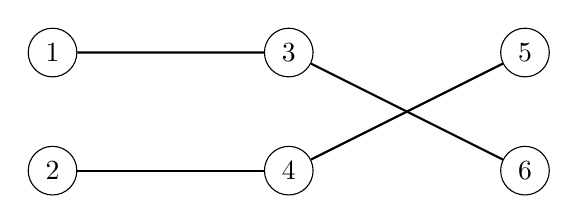
\begin{tikzpicture}[scale=1.5]
    % Draw nodes for V_1
    \node[circle, draw] (1) at (0, 1) {1};
    \node[circle, draw] (2) at (0, 0) {2};

    % Draw nodes for V_2
    \node[circle, draw] (3) at (2, 1) {3};
    \node[circle, draw] (4) at (2, 0) {4};

    % Draw nodes for V_3
    \node[circle, draw] (5) at (4, 1) {5};
    \node[circle, draw] (6) at (4, 0) {6};

    % Draw edges
    \draw[thick] (1) -- (3);
    \draw[thick] (2) -- (4);
    \draw[thick] (4) -- (5);
    \draw[thick] (3) -- (6);
\end{tikzpicture}
\caption{An example of a 3-partite graph}
\label{fig:d-partite}
\end{center}
\end{figure}

D-partite graphs are commonly seen in multi-dimensional matching problems, and algorithms for these graphs extend ideas from bipartite matching to higher dimensions.

\subsection{Matching}
A \textbf{matching} in a graph \( G = (V, E) \) is a subset \( M \subseteq E \) such that no two edges in \( M \) share a common vertex. In other words, a matching is a collection of edges where each vertex is incident to at most one edge.\cite{yadav2023advanced} For example, consider the following bipartite graph:
\[
V = \{1, 2, 3, 4, 5, 6\}, \quad E = \{\{1, 4\}, \{1, 5\}, \{2, 4\}, \{2, 6\}, \{3, 5\}, \{3, 6\}\}
\]

\begin{figure}[h]
\begin{center}
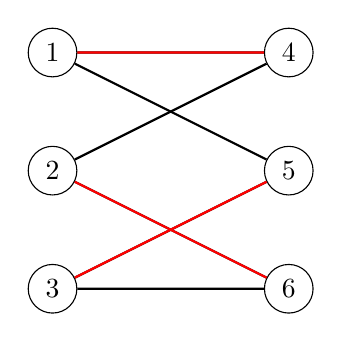
\begin{tikzpicture}[scale=1.5]
    % Draw nodes for set U
    \node[circle, draw] (u1) at (0, 1) {1};
    \node[circle, draw] (u2) at (0, 0) {2};
    \node[circle, draw] (u3) at (0, -1) {3};

    % Draw nodes for set V
    \node[circle, draw] (v1) at (2, 1) {4};
    \node[circle, draw] (v2) at (2, 0) {5};
    \node[circle, draw] (v3) at (2, -1) {6};

    % Draw all edges (undirected)
    \draw[thick] (u1) -- (v1); % Edge between 1 and 4
    \draw[thick] (u1) -- (v2); % Edge between 1 and 5
    \draw[thick] (u2) -- (v1); % Edge between 2 and 4
    \draw[thick] (u2) -- (v3); % Edge between 2 and 6
    \draw[thick] (u3) -- (v2); % Edge between 3 and 5
    \draw[thick] (u3) -- (v3); % Edge between 3 and 6

    % Highlight the matching edges
    \draw[thick, red] (u1) -- (v1); % Highlight matching edge between 1 and 4
    \draw[thick, red] (u2) -- (v3); % Highlight matching edge between 2 and 6
    \draw[thick, red] (u3) -- (v2); % Highlight matching edge between 3 and 5
\end{tikzpicture}
\caption{An example of a matching in a bipartite graph. The highlighted edges form a matching.}
\label{fig:matching}
\end{center}
\end{figure}

A valid matching is \( M = \{\{1, 4\}, \{2, 6\}, \{3, 5\}\} \).

Now consider the following 3-partite graph in Figure~\ref{fig:matching_d3}:
\[
V_1 = \{1, 2, 3\}, \quad V_2 = \{4, 5, 6\}, \quad V_3 = \{7, 8, 9\}
\]
\[
E = \{\{1, 4, 7\}, \{1, 5, 8\}, \{2, 5, 9\}, \{2, 6, 7\}, \{3, 6, 8\}, \{3, 7, 9\}\}
\]

\begin{figure}[h]
\begin{center}
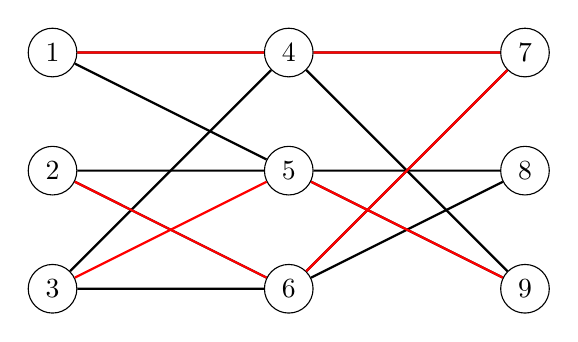
\begin{tikzpicture}[scale=1.5]
    % Draw nodes for set V1
    \node[circle, draw] (v11) at (0, 2) {1};
    \node[circle, draw] (v12) at (0, 1) {2};
    \node[circle, draw] (v13) at (0, 0) {3};

    % Draw nodes for set V2
    \node[circle, draw] (v21) at (2, 2) {4};
    \node[circle, draw] (v22) at (2, 1) {5};
    \node[circle, draw] (v23) at (2, 0) {6};

    % Draw nodes for set V3
    \node[circle, draw] (v31) at (4, 2) {7};
    \node[circle, draw] (v32) at (4, 1) {8};
    \node[circle, draw] (v33) at (4, 0) {9};

    % Draw edges between sets V1, V2, and V3
    \draw[thick] (v11) -- (v21) -- (v31); % Edge between 1, 4, and 7
    \draw[thick] (v11) -- (v22) -- (v32); % Edge between 1, 5, and 8
    \draw[thick] (v12) -- (v22) -- (v33); % Edge between 2, 5, and 9
    \draw[thick] (v12) -- (v23) -- (v31); % Edge between 2, 6, and 7
    \draw[thick] (v13) -- (v23) -- (v32); % Edge between 3, 6, and 8
    \draw[thick] (v13) -- (v21) -- (v33); % Edge between 3, 7, and 9

    % Highlight the matching edges
    \draw[thick, red] (v11) -- (v21) -- (v31); % Highlight matching edge between 1, 4, and 7
    \draw[thick, red] (v12) -- (v23) -- (v31); % Highlight matching edge between 2, 6, and 7
    \draw[thick, red] (v13) -- (v22) -- (v33); % Highlight matching edge between 3, 5, and 9
\end{tikzpicture}
\caption{An example of a matching in a 3-partite graph. The highlighted edges form a matching.}
\label{fig:matching_d3}
\end{center}
\end{figure}

A valid matching is \( M = \{\{1, 4, 7\}, \{2, 6, 7\}, \{3, 5, 8\}\} \).

\subsection{Paths, Cycles, and Augmenting Paths}

A \textbf{path} in a graph \( G = (V, E) \) is a sequence of vertices \( v_1, v_2, \dots, v_k \) such that for each \( i = 1, 2, \dots, k-1 \), the edge \( \{v_i, v_{i+1}\} \in E \). In directed graphs, the edges must be oriented in the direction of traversal. For example in Figure~\ref{fig:path}, in an undirected graph with vertices \( V = \{1, 2, 3, 4\} \) and edges \( E = \{\{1, 2\}, \{2, 3\}, \{3, 4\}\} \), the sequence \( 1, 2, 3, 4 \) forms a path. \cite{yadav2023advanced, cormen2009introduction}

\begin{figure}[h]
\begin{center}
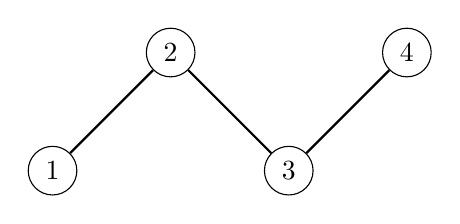
\begin{tikzpicture}[scale=1.5]
    % Draw nodes
    \node[circle, draw] (1) at (0, 0) {1};
    \node[circle, draw] (2) at (1, 1) {2};
    \node[circle, draw] (3) at (2, 0) {3};
    \node[circle, draw] (4) at (3, 1) {4};

    % Draw edges
    \draw[thick] (1) -- (2);
    \draw[thick] (2) -- (3);
    \draw[thick] (3) -- (4);
\end{tikzpicture}
\caption{Undirected Path in a Graph}
\label{fig:path}
\end{center}
\end{figure}

In a directed graph, the edges must be oriented. For example in Figure~\ref{fig:directed_path}, in a directed graph with vertices \( V = \{1, 2, 3, 4\} \) and edges \( E = \{(1, 2), (2, 3), (3, 4)\} \), the sequence \( 1 \to 2 \to 3 \to 4 \) forms a path.

\begin{figure}[h]
\begin{center}
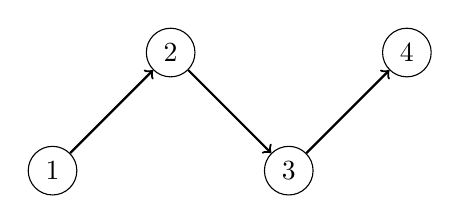
\begin{tikzpicture}[scale=1.5]
    % Draw nodes
    \node[circle, draw] (1) at (0, 0) {1};
    \node[circle, draw] (2) at (1, 1) {2};
    \node[circle, draw] (3) at (2, 0) {3};
    \node[circle, draw] (4) at (3, 1) {4};

    % Draw directed edges
    \draw[thick,->] (1) -- (2);
    \draw[thick,->] (2) -- (3);
    \draw[thick,->] (3) -- (4);
\end{tikzpicture}
\caption{Directed Path in a Graph}
\label{fig:directed_path}
\end{center}
\end{figure}

A \textbf{cycle} is a path that starts and ends at the same vertex. Formally, a cycle is a path \( v_1, v_2, \dots, v_k, v_1 \), where \( k \geq 3 \) and all the edges \( \{v_i, v_{i+1}\} \) for \( i = 1, 2, \dots, k-1 \), as well as \( \{v_k, v_1\} \), belong to \( E(G) \). For example in Figure~\ref{fig:cycle}, in an undirected graph with vertices \( V = \{1, 2, 3\} \) and edges \( E = \{\{1, 2\}, \{2, 3\}, \{3, 1\}\} \), the sequence \( 1, 2, 3, 1 \) forms a cycle. \cite{yadav2023advanced, cormen2009introduction}

\begin{figure}[h]
\begin{center}
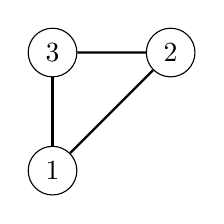
\begin{tikzpicture}[scale=1.5]
    % Draw nodes
    \node[circle, draw] (1) at (0, 0) {1};
    \node[circle, draw] (2) at (1, 1) {2};
    \node[circle, draw] (3) at (0, 1) {3};

    % Draw edges
    \draw[thick] (1) -- (2);
    \draw[thick] (2) -- (3);
    \draw[thick] (3) -- (1);
\end{tikzpicture}
\caption{Undirected Cycle in a Graph}
\label{fig:cycle}
\end{center}
\end{figure}

In a directed graph, a cycle can also be formed. For example in Figure~\ref{fig:directed_cycle}, in a directed graph with vertices \( V = \{1, 2, 3\} \) and edges \( E = \{(1, 2), (2, 3), (3, 1)\} \), the sequence \( 1 \to 2 \to 3 \to 1 \) forms a directed cycle.

\begin{figure}[h]
\begin{center}
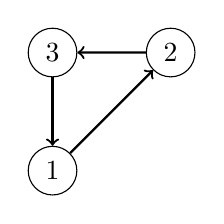
\begin{tikzpicture}[scale=1.5]
    % Draw nodes
    \node[circle, draw] (1) at (0, 0) {1};
    \node[circle, draw] (2) at (1, 1) {2};
    \node[circle, draw] (3) at (0, 1) {3};

    % Draw directed edges
    \draw[thick,->] (1) -- (2);
    \draw[thick,->] (2) -- (3);
    \draw[thick,->] (3) -- (1);
\end{tikzpicture}
\caption{Directed Cycle in a Graph}
\label{fig:directed_cycle}
\end{center}
\end{figure}

Let $G$ be a graph, and $M$ be a matching of $G$, then an \textbf{augmenting path} in $G$ alternates between edges in $M$ and edges that are not, beginning and ending at unmatched vertices.\cite{cormen2009introduction} For example in Figure~\ref{fig:augmenting_path}, consider a bipartite graph with vertex sets: 
\[ V = \{1, 2, 3, 4, 5, 6\}, \quad V_1 = \{1, 2, 3\}, \quad V_2 = \{4, 5, 6\}, \quad E = \{\{1, 4\}, \{2, 4\}, \{2, 5\}, \{3, 5\}, \{3, 6\}\} \] 

For the matching \( M = \{\{2, 4\}, \{3, 5\}\} \), the path \( 1 \to 4 \textcolor{red}{ \to} 2 \to 5 \textcolor{red}{ \to} 3 \to 6 \) forms an augmenting path because it starts at unmatched vertex 1, ends at unmatched vertex 6, and alternates between edges that are matched and unmatched. The red highlights indicate a matched edge.

\begin{figure}[h]
\begin{center}
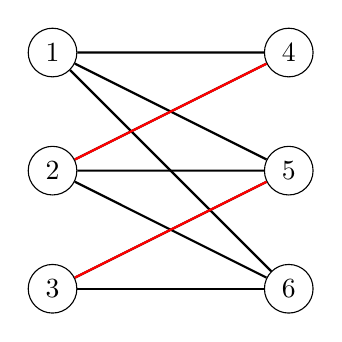
\begin{tikzpicture}[scale=1.5]
    % Draw nodes for V_1
    \node[circle, draw] (1) at (0, 2) {1};
    \node[circle, draw] (2) at (0, 1) {2};
    \node[circle, draw] (3) at (0, 0) {3};

    % Draw nodes for V_2
    \node[circle, draw] (4) at (2, 2) {4};
    \node[circle, draw] (5) at (2, 1) {5};
    \node[circle, draw] (6) at (2, 0) {6};

    % Draw edges
    \draw[thick] (1) -- (4);
    \draw[thick] (2) -- (4);
    \draw[thick] (2) -- (5);
    \draw[thick] (3) -- (5);
    \draw[thick] (3) -- (6);
    \draw[thick] (1) -- (5);
    \draw[thick] (2) -- (6);
    \draw[thick] (1) -- (6);

    % Draw matching edge (thicker and in red)
    \draw[thick, red] (2) -- (4);
    \draw[thick, red] (3) -- (5);
\end{tikzpicture}
\caption{Augmenting Path in a Bipartite Graph}
\label{fig:augmenting_path}
\end{center}
\end{figure}

\subsection{Connected Graphs}
A graph \( G = (V, E) \) is said to be \textbf{connected} if for every pair of vertices \( u, v \in V \), there exists a path from \( u \) to \( v \). In other words, all vertices in the graph are reachable from any other vertex \cite{yadav2023advanced, cormen2009introduction}.

If a graph is not connected, it is called \textbf{disconnected}. A disconnected graph consists of multiple \textbf{connected components}. A \textbf{connected component} of a graph is a maximal subgraph in which every pair of vertices is connected by a path. In other words, a connected component is a subset of the graph where there is a path between every pair of vertices, and no additional vertices or edges from outside the subset can be added without losing its connectivity.

For example, consider the graph \( G = (V, E) \) where:
\[
V = \{1, 2, 3, 4, 5\}, \quad E = \{\{1, 2\}, \{2, 3\}, \{4, 5\}\}
\]
The graph in Figure~\ref{fig:connected_graph} is disconnected, as there is no path between vertex 3 and vertex 4. This graph can be divided into two connected components:
\begin{itemize}
    \item Component 1: The vertices \( \{1, 2, 3\} \) with edges \( \{1, 2\}, \{2, 3\} \).
    \item Component 2: The vertices \( \{4, 5\} \) with edge \( \{4, 5\} \).
\end{itemize}

\begin{figure}[h]
\begin{center}
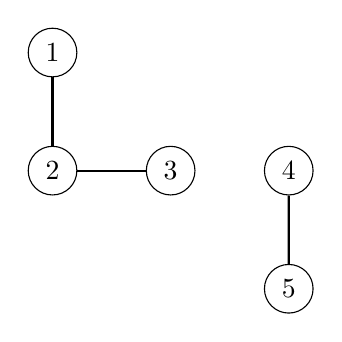
\begin{tikzpicture}[scale=1.5]
    % Draw nodes for the first connected component
    \node[circle, draw] (1) at (0, 1) {1};
    \node[circle, draw] (2) at (0, 0) {2};
    \node[circle, draw] (3) at (1, 0) {3};

    % Draw edges for the first connected component
    \draw[thick] (1) -- (2);
    \draw[thick] (2) -- (3);

    % Draw nodes for the second connected component
    \node[circle, draw] (4) at (2, 0) {4};
    \node[circle, draw] (5) at (2, -1) {5};

    % Draw edges for the second connected component
    \draw[thick] (4) -- (5);
\end{tikzpicture}
\caption{An example of a disconnected graph with two connected components.}
\label{fig:connected_graph}
\end{center}
\end{figure}

\subsection{Complete Graphs}
A \textbf{complete graph} \( K_n \) is a graph where every pair of distinct vertices is connected by an edge. Formally, a complete graph with \( n \) vertices has \( \frac{n(n-1)}{2} \) edges, as all possible pairs of vertices are connected. For example, the complete graph \( K_3 \) in Figure~\ref{fig:complete_graph} has the following edges:
\[
V = \{1, 2, 3\}, \quad E = \{\{1, 2\}, \{1, 3\}, \{2, 3\}\}
\]
This results in 3 edges, which is the maximum number of edges in a graph with 3 vertices.

\begin{figure}[h]
\begin{center}
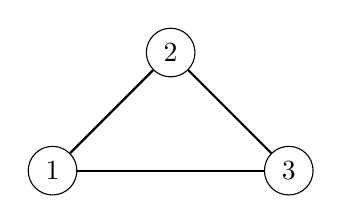
\begin{tikzpicture}[scale=1.5]
    % Draw nodes
    \node[circle, draw] (1) at (0, 0) {1};
    \node[circle, draw] (2) at (1, 1) {2};
    \node[circle, draw] (3) at (2, 0) {3};

    % Draw edges (undirected)
    \draw[thick] (1) -- (2); % Edge between 1 and 2
    \draw[thick] (2) -- (3); % Edge between 2 and 3
    \draw[thick] (1) -- (3); % Edge between 1 and 3
\end{tikzpicture}
\caption{An example of the complete graph \( K_3 \), where every pair of distinct vertices is connected by an edge.}
\label{fig:complete_graph}
\end{center}
\end{figure}

Complete graphs are often used in theoretical explorations of matching, covering, and flow problems, as they provide the maximum number of potential connections between vertices \cite{yadav2023advanced, cormen2009introduction}.

\subsubsection*{Complete \( d \)-Partite Graphs}

A \textbf{complete \( d \)-partite graph} is a graph where the vertex set \( V \) is partitioned into \( d \) disjoint sets \( V_1, V_2, \dots, V_d \), and every vertex in one set is connected to every vertex in the other sets, but there are no edges between vertices within the same set.

For \( d = 2 \), this is simply a \textbf{complete bipartite graph}, where the vertex set \( V \) is divided into two disjoint sets \( V_1 \) and \( V_2 \), and every vertex in \( V_1 \) is connected to every vertex in \( V_2 \), but there are no edges between vertices within \( V_1 \) or within \( V_2 \). A complete bipartite graph is denoted as \( K_{m,n} \), where \( m \) and \( n \) are the sizes of the two disjoint sets \( V_1 \) and \( V_2 \), respectively. The number of edges in \( K_{m,n} \) is given by \( m \times n \).

For example in Figure~\ref{fig:complete_bipartite}, consider the complete bipartite graph \( K_{3,3} \), where:
\[
V_1 = \{1, 2, 3\}, \quad V_2 = \{4, 5, 6\}, \quad E = \{\{1,4\}, \{1,5\}, \{1,6\}, \{2,4\}, \{2,5\}, \{2,6\}, \{3,4\}, \{3,5\}, \{3,6\}\}.
\]

\begin{figure}[h]
\begin{center}
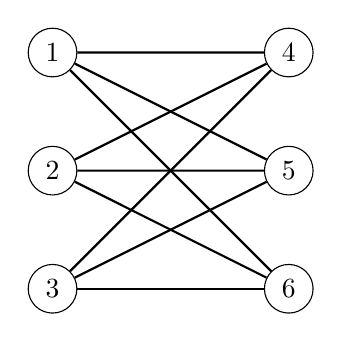
\begin{tikzpicture}[scale=1.5, every node/.style={circle, draw}]
    % Nodes for the first partition
    \node (1) at (0, 2) {1};
    \node (2) at (0, 1) {2};
    \node (3) at (0, 0) {3};
    
    % Nodes for the second partition
    \node (4) at (2, 2) {4};
    \node (5) at (2, 1) {5};
    \node (6) at (2, 0) {6};
    
    % Edges between the two partitions
    \draw[thick] (1) -- (4);
    \draw[thick] (1) -- (5);
    \draw[thick] (1) -- (6);
    \draw[thick] (2) -- (4);
    \draw[thick] (2) -- (5);
    \draw[thick] (2) -- (6);
    \draw[thick] (3) -- (4);
    \draw[thick] (3) -- (5);
    \draw[thick] (3) -- (6);
\end{tikzpicture}
\caption{A complete bipartite graph \( K_{3,3} \) with two partitions \( V_1 = \{1, 2, 3\} \) and \( V_2 = \{4, 5, 6\} \). Every vertex in \( V_1 \) is connected to every vertex in \( V_2 \).}
\label{fig:complete_bipartite}
\end{center}
\end{figure}

For \( d > 2 \), the complete \( d \)-partite graph consists of \( d \) disjoint vertex sets \( V_1, V_2, \dots, V_d \), and every vertex in \( V_i \) is connected to every vertex in all other sets \( V_j \) (for \( i \neq j \)), but there are no edges between vertices within the same set. The number of edges in a complete \( d \)-partite graph is the sum of the edges between each pair of sets, calculated as:
\[
\text{Total edges} = \sum_{1 \leq i < j \leq d} |V_i| \times |V_j|
\]
This formula counts the edges between each pair of disjoint sets.

\subsection{Graph Representations}
A graph \( G = (V, E) \) can be represented as an adjacency matrix or as a collection of adjacency lists. If a graph is dense (\(|E|\) is close to \(|V|^2\)), an adjacency matrix is used. If a graph is sparse (\(|E|\) is much less than \(|V|^2\)), an adjacency list is the more efficient choice. \cite{yadav2023advanced} \cite{cormen2009introduction}

\subsubsection*{Adjacency Matrix}
The \textbf{adjacency matrix} of a bipartite graph \( G = (V, E) \) with two sets of vertices is an \( n \times m \) matrix \( A \) where each entry \( A_{ij} \) is defined as follows:
\[
A_{ij} =
\begin{cases}
1, & \text{if } \{u_i, v_j\} \in E, and \\
0, & \text{otherwise}
\end{cases}
\]
For example, consider the bipartite graph \( G = (V, E) \) where:
\[
V_1 = \{1, 2\}, \quad V_2 = \{3, 4\}, \quad E = \{\{1, 3\}, \{1, 4\}, \{2, 4\}\}
\]
The adjacency matrix \( A \) for this bipartite graph is:
\[
A =
\begin{bmatrix}
1 & 1 \\
0 & 1 
\end{bmatrix}
\]
where rows correspond to vertices in \( V_1 \) and columns correspond to vertices in \( V_2 \).

\begin{figure}[h]
\begin{center}
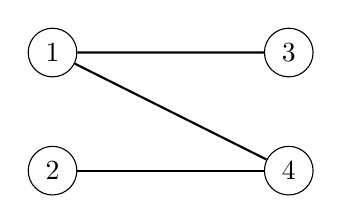
\begin{tikzpicture}[scale=1.5]
    % Draw nodes for V1
    \node[circle, draw] (1) at (0, 1) {1};
    \node[circle, draw] (2) at (0, 0) {2};

    % Draw nodes for V2
    \node[circle, draw] (3) at (2, 1) {3};
    \node[circle, draw] (4) at (2, 0) {4};

    % Draw edges
    \draw[thick] (1) -- (3);
    \draw[thick] (1) -- (4);
    \draw[thick] (2) -- (4);
\end{tikzpicture}
\caption{Adjacency Matrix Representation of a Bipartite Graph}
\label{fig:adj_matrix}
\end{center}
\end{figure}

Adjacency matrices are used to quickly tell if there is an edge connecting two given vertices. The adjacency matrix is particularly useful in algorithms where matrix multiplication or graph traversal plays a significant role, such as in finding augmenting paths for matchings. The amount of memory required is $\Theta(V^2)$, which is independent of the number of edges on the graph.

\subsubsection*{Adjacency List}
The \textbf{adjacency list} of a bipartite graph \( G = (V, E) \) is a collection of lists, one for each vertex, where each list contains the vertices adjacent to that vertex.

For example, consider the bipartite graph \( G = (V, E) \) where:
\[
V_1 = \{1, 2\}, \quad V_2 = \{3, 4\}, \quad E = \{\{1, 3\}, \{1, 4\}, \{2, 4\}\}
\]
The adjacency list for the following bipartite graph is:
\[
\text{Adjacency List:}
\begin{array}{l}
1: \{3, 4\} \\
2: \{4\} \\
3: \{1\} \\
4: \{1, 2\}
\end{array}
\]

\begin{figure}[h]
\begin{center}
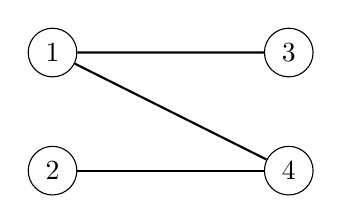
\begin{tikzpicture}[scale=1.5]
    % Draw nodes for V1
    \node[circle, draw] (1) at (0, 1) {1};
    \node[circle, draw] (2) at (0, 0) {2};

    % Draw nodes for V2
    \node[circle, draw] (3) at (2, 1) {3};
    \node[circle, draw] (4) at (2, 0) {4};

    % Draw edges
    \draw[thick] (1) -- (3);
    \draw[thick] (1) -- (4);
    \draw[thick] (2) -- (4);
\end{tikzpicture}
\caption{Adjacency List Representation of a Bipartite Graph}
\label{fig:adj_list}
\end{center}
\end{figure}

This representation is efficient for sparse graphs and is widely used in graph traversal algorithms. For example, finding an augmenting path in matching algorithms can be performed efficiently using adjacency lists. The amount of memory required is $\Theta(V+E)$.

\subsection{Berge's Theorem}
It is not \textit{a priori} easy to determine whether a given matching is maximum; the obvious way to do so involves searching for all other matchings.
Berge's theorem gives an easier method for general graphs:

\begin{theorem}\label{berge} \cite{berge}
    A matching $M$ in a graph $G$ is a maximum matching if and only if has no augmenting path.
\end{theorem}

Consider the matching $\{(2, 4), (3, 5)\}$ in the following graph. It is not maximum; it has the augmenting path (1,4), (4, 2), (2, 5), (5, 3), (3, 6).

\begin{center}
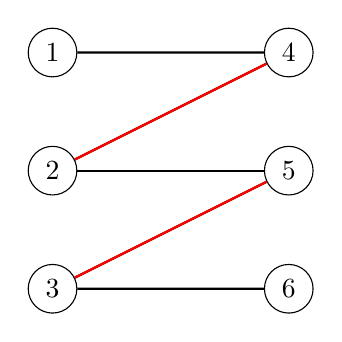
\begin{tikzpicture}[scale=1.5]
    % Draw nodes for set U
    \node[circle, draw] (u1) at (0, 1) {1};
    \node[circle, draw] (u2) at (0, 0) {2};
    \node[circle, draw] (u3) at (0, -1) {3};

    % Draw nodes for set V
    \node[circle, draw] (v1) at (2, 1) {4};
    \node[circle, draw] (v2) at (2, 0) {5};
    \node[circle, draw] (v3) at (2, -1) {6};

    % Draw all edges (undirected)
    \draw[thick] (u1) -- (v1); % Edge between 1 and 4
    \draw[thick] (u2) -- (v1); % Edge between 2 and 4
    \draw[thick] (u2) -- (v2); % Edge between 2 and 5
    \draw[thick] (u3) -- (v2); % Edge between 3 and 5
    \draw[thick] (u3) -- (v3); % Edge between 3 and 6

    % Highlight the matching edges
    \draw[thick, red] (u2) -- (v1); % Highlight matching edge between 2 and 4
    \draw[thick, red] (u3) -- (v2); % Highlight matching edge between 3 and 5
\end{tikzpicture}
\label{fig:berge_example}
\end{center}

\begin{proof}[Proof of \Cref{berge}]
Suppose $M$ has an augmenting path $P$ and let us prove $M$ is not maximum. It may be assumed that $P$ is simple.
We claim the symmetric difference $(M - P) \cup (P - M)$ is a matching.
For example, suppose $e$ and $e'$ are distinct edges of $(M - P) \cup (P - M)$ sharing a vertex. 

There are three cases:
(1) Both are in $M$: We reach a contradiction since $M$ is a matching.

(2) Both are in $P - M$: then $e$ and $e'$ are successive edges since $P$ is simple.
As $P$ is augmenting, one of $e, e'$ is in $M$, a contradiction.

(3) One (say $e$) is in $M - P$ and the other (say $e'$) is in $P - M$.
Let $v$ be the vertex shared by $e$ and $e'$.
Since $e \in M$ and $P$ is augmenting, $v$ is not an endpoint of $P$.
So there is another edge $e'' \in P$ that also contains $v$.
Observe that $e$ and $e''$ are distinct vertices of $M$ containing $v$ for a contradiction.

Also, $|(M - P) \cup (P - M)| = (|M| - \frac{|P| - 1}{2}) + \frac{|P| + 1}{2} = |M| + 1$ to conclude.

In the other direction,  suppose $M$ has no augmenting path.
To show that $M$ is maximum, let $M'$ be another matching of $G$.
Consider the symmetric difference graph $(M - M')\cup (M' - M)$.
The connected components of $(M - M')\cup (M' - M)$ are simple paths and even cycles alternating between edges in $M$ and $M'$. The assumption on $M$ ensures each of the former start or end with an edge of $M$ (for otherwise they would be an augmenting path for $M$).
Thus each component has intersection with $M$ at least as large as with $M'$, showing $|M| - |M\cap M'| = |M - M'| \geq |M' - M| = |M'| - |M\cap M'|$ i.e. $|M| \geq |M'|$.
\end{proof}

The proof of Theorem \Cref{berge} gives a strategy to find a maximum matching: beginning with a matching (such as $\varnothing$), repeatedly finding augmenting paths and taking symmetric differences until there are no more.
This strategy is key to various algorithms in Chapter 4.